% Enable warnings about problematic code
\RequirePackage[l2tabu, orthodox]{nag}

\documentclass{WeSTassignment}

% The lecture title, e.g. "Web Information Retrieval".
\lecture{Introduction to Web Science}
% The names of the lecturer and the instructor(s)
\author{%
  Prof. Dr.~Steffen~Staab\\{\normalsize\mailto{staab@uni-koblenz.de}} \and
  Ren{\'e}~Pickhardt\\{\normalsize\mailto{rpickhardt@uni-koblenz.de}} \and
   Korok~Sengupta\\{\normalsize\mailto{koroksengupta@uni-koblenz.de}}
}
% Assignment number.
\assignmentnumber{3}
% Institute of lecture.
\institute{%
  Institute of Web Science and Technologies\\%
  Department of Computer Science\\%
  University of Luxembourg%
}
% Date until students should submit their solutions.
\datesubmission{November 16, 2016, 10:00 a.m.}
% Date on which the assignments will be discussed in the tutorial.
\datetutorial{November 18, 2016, 12:00 p.m.}

% Set langauge of text.
\setdefaultlanguage[
  variant = american, % Use American instead of Britsh English.
]{english}

% Specify bib file location.
\addbibresource{bibliography.bib}

% For left aligned centerd boxes
% see http://tex.stackexchange.com/a/25591/75225
\usepackage{varwidth}

% ==============================================================================
% Document

\begin{document}

\maketitle

The main objective of this assignment is for you understand different concepts that are associated with the "Web". In this assignment we cover two topics: 1) DNS \& 2) Internet. 

These tasks are not always specific to \enquote{Introduction to Web Science}.
For all the assignment questions that require you to write a code, make sure to include the code in the answer sheet, along with a separate python file. Where screen shots are required, please add them in the answers directly and not as separate files.\\ \\ 

%Please mention your team Names here: 
Team Name: \textbf{papa}
Brigitte Aznar \\
Bonasmitha Behura \\
Ilia Tugushi

% ------------------------------------------------------------------------------

\section{DIG Deeper (5 Points)}

Assignment 1 started with you googling certain basic tools and one of them was "\emph{dig}". 
\begin{enumerate}
\item Now using that dig command, find the IP address of \url{ www.uni-koblenz-landau.de}
\item In the result, you will find "SOA". What is SOA? 
\item Copy the SOA record that you find in your answer sheet and explain each of the components of SOA with regards to your find. Merely integrating answers from the internet wont fetch you points.  

\end{enumerate}
Try the experiment once from University network and once from Home network and see if you can find any differences and if so, clarify why. 

\textbf{Answers:}\\

\begin{enumerate}
\item The IP address is 141.26.200.8 \\
\begin{figure}[h]
  \centering
  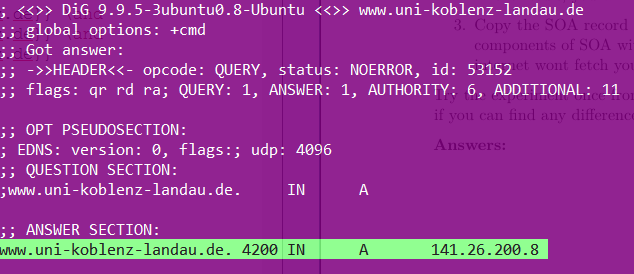
\includegraphics{dig.png}
   \caption{Dig IP address}
     \label{fig:dig} 
\end{figure}
\item SOA stands for Start of Authority 
\end{enumerate}

% ------------------------------------------------------------------------------

\section{Exploring DNS (10 Points)}

In the first part of this assignment you were asked to develop a simple TCP Client Server. Now, using \textbf{that} client server setup.
This time a url should be send to the server and the server will split the url into the following:\\ 

\url{http://www.example.com:80/path/to/myfile.html?key1=value1&key2=value2#InTheDocument}

\begin{enumerate}
\item Protocol
\item Domain
\item Sub-Domain
\item Port number
\item Path
\item Parameters
\item Fragment
\end{enumerate}

The Protocol for sending the URL will be a string terminated with \backslash r \backslash n.

P.S.: You are \textbf{not} allowed to use libraries like \texttt{urlparse} for this question. You will also not use "Regular Expressions" for this. 

\textbf{Answer:} 

\begin{lstlisting}
import socket
import json

def Main():

    socket_server = socket.socket()
    socket_server.bind(('localhost', 8080))

    socket_server.listen(1)
    conn, addr = socket_server.accept()
    print("Connection from: " + str(addr))
    data = conn.recv(1024)
    data = data.decode('utf-8')
    if not data:
        print('no data received')
        return

    url        = data.split(".")
    colon      = url[0].split(":")
    protocol   = colon[0]
    domain     = url[2]
    domain     = domain.split(":")
    domain     = domain[0]
    subdomain  = url[1]

    port       = url[2].split(":")
    path       = port[1]
    port       = port[1].split("/")
    port       = port[0]
    path       = path.split("80")
    path       = path[1]
    tail       = url[3].split("?")
    tail       = tail[1].split("#")
    params     = tail[0]
    fragment   = tail[1]
    fragment   = fragment.split("\\")
    fragment   = fragment[0]

    print('Protocol: ', protocol)
    print('Subdomain: ', subdomain)
    print('Domain: ', domain)
    print('Port: ', port)
    print('Patha: ', path)
    print('Params: ', params)
    print('Fragments: ', fragment)
    conn.close()


if __name__ == '__main__':
    Main()
\end{lstlisting}
\begin{figure}[h]
  \centering
  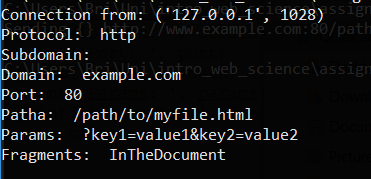
\includegraphics{splitting_url.png}
   \caption{URL parts}
     \label{fig:dig} 
\end{figure}

% ------------------------------------------------------------------------------


\section{DNS Recursive Query Resolving (5 Points)}

You have solved the "Routing Table" question in Assignment 2. We updated the routing tables once more. resulting in the following tables creating the following topology 

% Please add the following required packages to your document preamble:
% \usepackage[normalem]{ulem}
% \useunder{\uline}{\ul}{}
\begin{table}[h]
\centering
\caption{Routing Table}
\label{routing table}
\scalebox{0.8}{
\begin{tabular}{|c|c|c|c|c|c|c|c|c|c|c|}
\hline
\multicolumn{3}{|c|}{\textbf{Router1}} &        & \multicolumn{3}{c|}{\textbf{Router2}} &        & \multicolumn{3}{c|}{\textbf{Router3}} \\ \hline
Destination  & Next Hop    & Interface &        & Destination & Next Hop    & Interface &        & Destination  & Next Hop   & Interface \\ \hline
67.0.0.0     & 67.68.3.1   & eth 0     &        & 205.30.7.0  & 205.30.7.1  & eth 0     &        & 205.30.7.0   & 205.30.7.2 & eth 0     \\ \hline
62.0.0.0     & 62.4.31.7   & eth 1     &        & 156.3.0.0   & 156.3.0.6   & eth 1     &        & 88.0.0.0     & 88.6.32.1  & eth 1     \\ \hline
88.0.0.0     & 88.4.32.6   & eth 2     &        & 26.0.0.0    & 26.3.2.1    & eth 2     &        & 25.0.0.0     & 25.03.1.2  & eth 2     \\ \hline
141.71.0.0   & 141.71.20.1 & eth 3     &        & 141.71.0.0  & 141.71.26.3 & eth 3     &        & 121.0.0.0    & 121.0.3.1  & eth 3     \\ \hline
26.0.0.0     & 141.71.26.3 & eth3      &        & 67.0.0.0    & 141.71.20.1 & eth 3     &        & 156.3.0.0    & 205.30.7.1 & eth 0     \\ \hline
156.3.0.0    & 88.6.32.1   & eth 2     &        & 62.0.0.0    & 141.71.20.1 & eth 3     &        & 26.0.0.0     & 205.30.7.1 & eth 0     \\ \hline
205.30.7.0   & 141.71.26.3 & eth 3     &        & 88.0.0.0    & 141.71.20.1 & eth 3     &        & 141.71.0.0   & 205.30.7.1 & eth 0     \\ \hline
25.0.0.0     & 88.6.32.1   & eth 2     &        & 25.0.0.0    & 205.30.7.2  & eth 0     &        & 67.0.0.0     & 88.4.32.6  & eth 1     \\ \hline
121.0.0.0    & 88.6.32.1   & eth 2     &        & 121.0.0.0   & 205.30.7.2  & eth 0     &        & 62.0.0.0     & 88.4.32.6  & eth 1     \\ \hline
\end{tabular}
}
\end{table}

\begin{figure}[h]
  \centering
  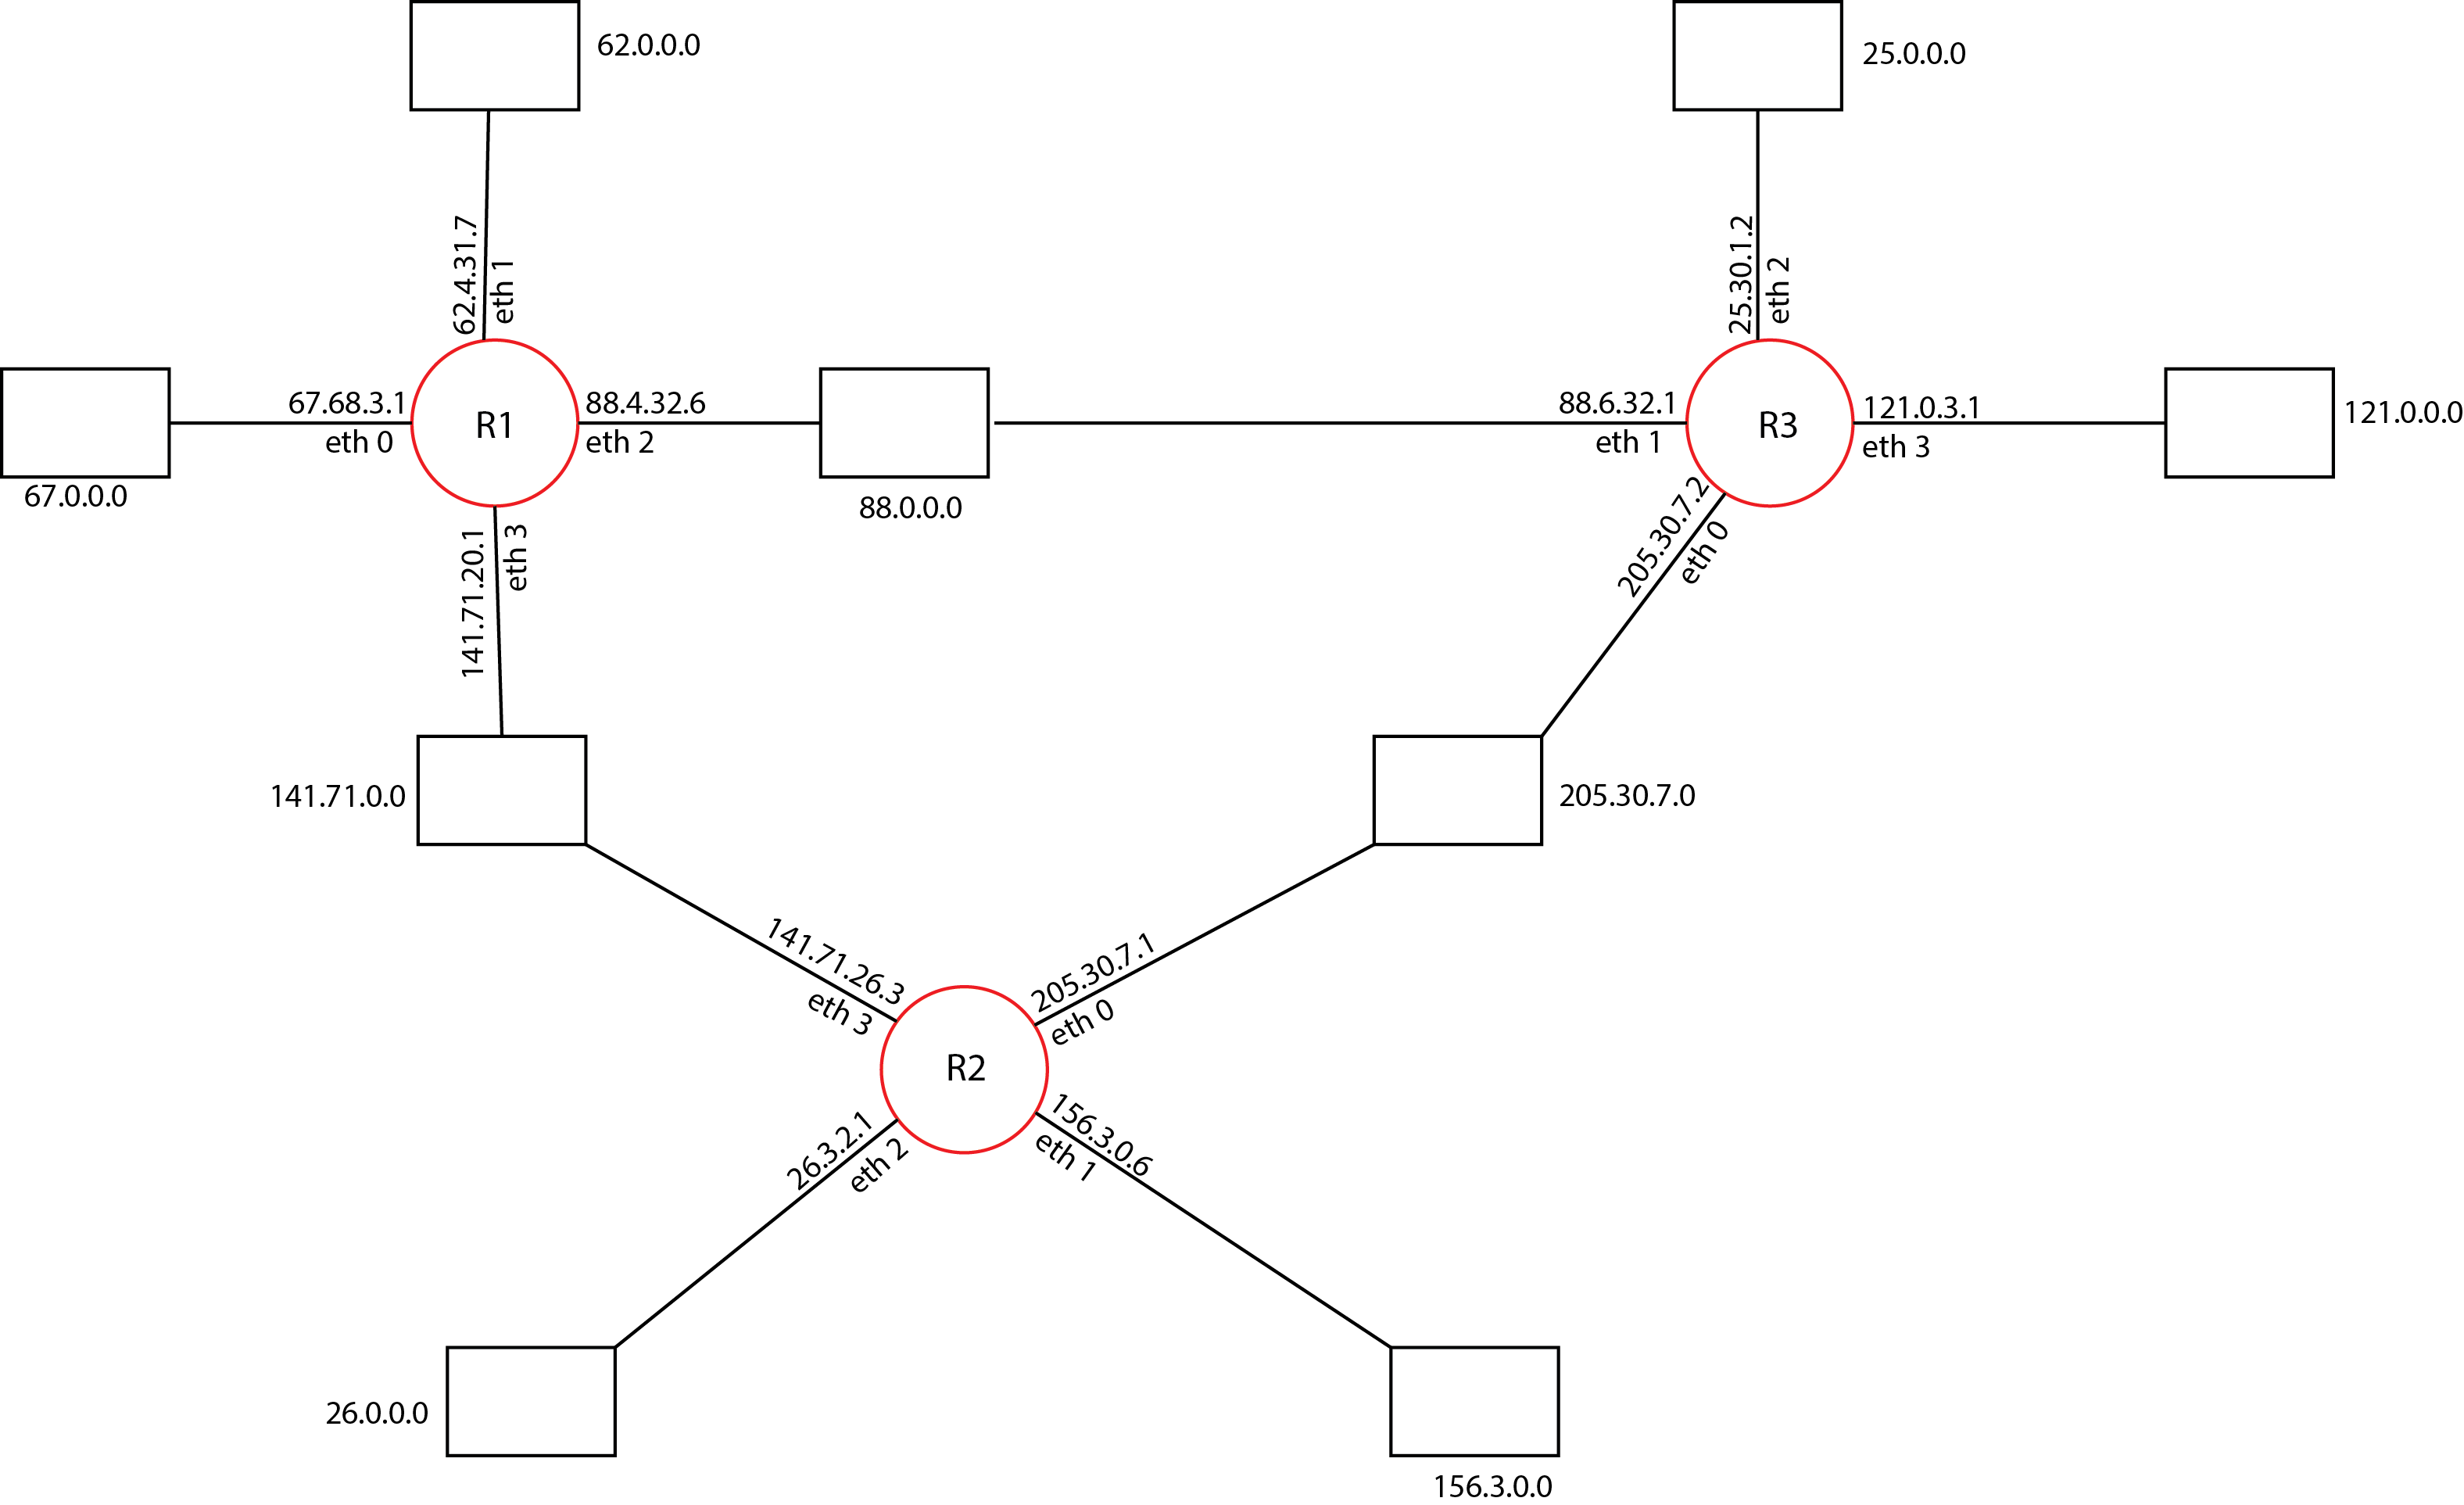
\includegraphics[scale=0.45]{ass3_DNS.png}
   \caption{DNS Routing Network}
     \label{fig:routing} 
\end{figure}

Let us asume a client with the following ip address 67.4.5.2 wants to resolve the following domain  \texttt{subdomain.webscienceexampledomain.com} using the DNS.

You can further assume the root name server has the IP address of 25.8.2.1 and the name-server for \texttt{webscienceexampledomain.com} has the IP address 156.3.20.2. 
Finally the sub-domain is handled by a name server with the IP of 26.155.36.7. 

Please explain how the traffic flows through the network in order to resolve the recursive DNS query. You can assume ARP tables are cached so that no ARP-requests have to be made. 

\textbf{Hint: You can start like this}: 

67.4.5.2 creates an IP packet with the source address XXXXXX an destination address YYYYY inside there is the DNS request. This IP packet is send as an ethernet frame to ZZZZZ. 
ZZZZZ receives the frame and forwards the encapsulated IP packet to ....

Also you can assume the DNS requests and responses will fit inside one IP packet. You also don't have to write down the specific DNS requests and responses in hex. 


% ------------------------------------------------------------------------------




\makefooter

\end{document}
